% ======================================================================
%  Chapter 17 — Loss, Gain, and Non-Hermitian Topology  (EXPANDED)
% ======================================================================

\section{When Hermiticity fails}
\label{sec:ch17-fails}

The entire topological framework of Parts~I--IV rests on the Hermiticity
of the Maxwell eigenvalue problem: the material matrix $\Mmat$ is
Hermitian ($\Mmat=\Mmat^\dagger$), the energy inner product is positive
definite, eigenfrequencies are real, and modes are orthogonal.  Real
photonic systems, however, always have losses (absorption, radiation
leakage) and sometimes gain (from pumped active media).  When these
effects are significant, the material matrix is no longer Hermitian, and
the standard topological theory must be revised.

This chapter examines what survives, what breaks, and what new
phenomena emerge when the Maxwell system is non-Hermitian
\cite{gong2018topologicala,ozawa2018topological}.

\section{Non-Hermitian Maxwell equations}
\label{sec:ch17-nh-maxwell}

\subsection{Complex material parameters}
\label{sec:ch17-complex}

In a lossy medium, the permittivity and permeability acquire imaginary
parts: $\varepsilon(\omega)=\varepsilon'(\omega)+\ii\varepsilon''(\omega)$.
With our time convention $\ee^{-\ii\omega t}$, absorption corresponds
to $\varepsilon''>0$ (energy is removed from the field), while gain
corresponds to $\varepsilon''<0$.

The material matrix $\Mmat$ is no longer Hermitian:
$\Mmat\neq\Mmat^\dagger$.  Specifically, the anti-Hermitian part
$\Mmat_A=(\Mmat-\Mmat^\dagger)/(2\ii)$ is nonzero and represents
the loss/gain distribution.

\subsection{Complex eigenfrequencies}
\label{sec:ch17-complex-eigenfreq}

The Maxwell eigenvalue equation $\Maxop\emfield=\omega\Mmat\emfield$
now has \emph{complex} eigenfrequencies:
$\omega_n=\omega_n'-\ii\gamma_n$, where $\omega_n'$ is the oscillation
frequency and $\gamma_n$ is the decay (or growth) rate:
\begin{itemize}
  \item $\gamma_n>0$: the mode decays (lossy).
  \item $\gamma_n<0$: the mode grows (amplified).
  \item $\gamma_n=0$: the mode is at the lasing threshold.
\end{itemize}

The complex eigenfrequencies trace curves in the complex $\omega$-plane
as the Bloch wavevector $\kvec$ varies over the Brillouin zone.

\subsection{Breakdown of the energy inner product}
\label{sec:ch17-breakdown}

The electromagnetic energy inner product
$\emip{\emfield_1}{\emfield_2}=\int\emfield_1^\dagger\Mmat\emfield_2
\,\dd^d r$ is no longer positive definite when $\Mmat$ has a
significant anti-Hermitian part.  The physical consequences are:
\begin{enumerate}
  \item The ``energy'' of a mode can be negative, zero, or complex.
  \item The modes are not orthogonal under $\langle\cdot|\Mmat|\cdot\rangle$.
  \item The Berry connection defined with this inner product is
  complex-valued, not real.
  \item The standard Chern-number formula may give non-integer values.
\end{enumerate}

\section{Biorthogonal modes}
\label{sec:ch17-biorthogonal} \cite{kunst2018biorthogonal}

\subsection{Right and left eigenmodes}
\label{sec:ch17-right-left}

For a non-Hermitian operator, one must distinguish between \emph{right}
eigenmodes $\emfield_n^R$ and \emph{left} eigenmodes $\emfield_n^L$:
\begin{align}
  \Mmat^{-1}\Maxop\,\emfield_n^R &= \omega_n\,\emfield_n^R\,,
  \label{eq:ch17-right}\\
  (\Mmat^{-1}\Maxop)^\dagger\emfield_n^L &= \omega_n^*\,\emfield_n^L\,.
  \label{eq:ch17-left}
\end{align}
The left and right eigenmodes satisfy a biorthogonality relation:
\begin{equation}\label{eq:ch17-biorthogonal}
  \int(\emfield_n^L)^\dagger\,\Mmat\,\emfield_m^R\,\dd^d r
  = N_n\,\delta_{nm}\,,
\end{equation}
where $N_n$ is a normalisation constant that can be complex.

\subsection{The biorthogonal Berry connection}
\label{sec:ch17-biorthogonal-berry}

The Berry connection must be modified to use the biorthogonal inner
product:
\begin{equation}\label{eq:ch17-nh-berry}
  \boxed{%
  \Aberry_n^{\mathrm{NH}}(\kvec)
  = \ii\frac{\int(\mathbf{u}_n^L)^\dagger\,\Mmat\,
  \nabla_\kvec\mathbf{u}_n^R\,\dd^d r}
  {\int(\mathbf{u}_n^L)^\dagger\,\Mmat\,\mathbf{u}_n^R\,\dd^d r}\,,}
\end{equation}
where $\mathbf{u}_n^{R,L}$ are the cell-periodic parts of the right
and left Bloch eigenmodes.

This connection is generally \emph{complex-valued} (unlike the
Hermitian case where $\Aberry$ is real).  Its real part contributes to
the Chern number, while its imaginary part is related to the
$\kvec$-dependence of the mode decay rate.

\section{Exceptional points}
\label{sec:ch17-ep}

\subsection{Definition and structure}
\label{sec:ch17-ep-def}

The most dramatic non-Hermitian phenomenon is the \emph{exceptional
point} (EP) \cite{ozawa2018topological}: a point in parameter space where two (or more)
eigenvalues \emph{and} their eigenvectors coalesce.  At an EP, the
operator becomes \emph{defective}: it cannot be diagonalised and
instead has a Jordan-block form.

For a $2\times 2$ non-Hermitian matrix, the canonical form at an EP is
\begin{equation}\label{eq:ch17-ep-jordan}
  H_{\mathrm{EP}} = \omega_0\mathbf{I} + \begin{pmatrix}
    0 & 1 \\ 0 & 0
  \end{pmatrix}.
\end{equation}
This is fundamentally different from a Hermitian degeneracy (Dirac
point), where the eigenvectors remain linearly independent even though
the eigenvalues coincide.

\subsection{A concrete photonic example}
\label{sec:ch17-ep-example}

Consider two coupled optical resonators with resonance frequencies
$\omega_1$ and $\omega_2$, coupling strength $J$, and individual
loss/gain rates $\gamma_1$ and $\gamma_2$.  The effective Hamiltonian
is
\begin{equation}\label{eq:ch17-coupled-resonators}
  H = \begin{pmatrix}
    \omega_1-\ii\gamma_1 & J \\
    J & \omega_2-\ii\gamma_2
  \end{pmatrix}.
\end{equation}
The eigenvalues are
\begin{equation}\label{eq:ch17-coupled-eigenvalues}
  \omega_\pm = \frac{(\omega_1+\omega_2)-\ii(\gamma_1+\gamma_2)}{2}
  \pm\sqrt{J^2+\Bigl(\frac{\delta\omega-\ii\delta\gamma}{2}\Bigr)^2}\,,
\end{equation}
where $\delta\omega=\omega_1-\omega_2$ and
$\delta\gamma=\gamma_1-\gamma_2$.

An exceptional point occurs when the discriminant vanishes:
\begin{equation}\label{eq:ch17-ep-condition}
  J^2 + \Bigl(\frac{\delta\omega-\ii\delta\gamma}{2}\Bigr)^2 = 0
  \quad\Longrightarrow\quad
  J = \frac{|\delta\gamma|}{2}\,,\quad \delta\omega=0\,
\end{equation}
The displayed formula above follows the convention and normalisation used in \cite{wan2011time}.
At this point, both eigenvalues and eigenvectors coalesce.

\subsection{Square-root behaviour near an EP}
\label{sec:ch17-ep-sqrt}

Near the EP, the eigenvalue splitting scales as the \emph{square root}
of the perturbation:
\begin{equation}\label{eq:ch17-ep-splitting}
  \omega_\pm \approx \omega_{\mathrm{EP}} \pm \sqrt{\delta}\,,
\end{equation}
where $\delta$ parametrises the distance from the EP.  This
sub-linear sensitivity (as opposed to the linear splitting at a Dirac
point) has been exploited for sensing applications:  small perturbations
produce disproportionately large frequency splittings near an EP.

\subsection{Topological properties of exceptional points}
\label{sec:ch17-ep-topology}

Exceptional points carry their own topological invariants, distinct from
the Chern numbers of Hermitian band theory:

\paragraph{Eigenvalue exchange.}
Encircling an EP in parameter space causes the two eigenvalues to
\emph{exchange}: $\omega_+\to\omega_-$ and $\omega_-\to\omega_+$.
After two circuits, the eigenvalues return to their original values.
This permutation has a topological winding number of $\pm\frac{1}{2}$.

\paragraph{Eigenvector monodromy.}
Under the same circuit, the eigenvectors acquire a geometric phase and
exchange: $|\psi_+\rangle\to\ee^{\ii\phi}|\psi_-\rangle$.  This
nontrivial monodromy is a direct consequence of the branch-point
structure of the square root in \eqref{eq:ch17-ep-splitting}.

\paragraph{Discriminant number.}
The discriminant $\Delta=(\omega_+-\omega_-)^2$ vanishes at the EP.
The winding of $\arg(\Delta)$ around the EP is $2\pi$, corresponding
to a discriminant number of $+1$ or $-1$.

The square-root branch-point topology is visualised in
Figure~\ref{fig:ch17-ep-riemann}.  Panel~(a) maps the principal argument
$\mathrm{Arg}(\sqrt{\lambda})$ over the complex $\lambda$-plane, where
$\lambda$ parametrises the eigenvalue discriminant.  Because the principal
square root halves the argument, the phase ranges over $(-\pi/2,\,\pi/2]$ and
exhibits a discontinuous jump across the branch cut on the negative real axis.
The exceptional point sits at the origin, where the two Riemann sheets meet.
Panel~(b) shows the concrete physical realisation in a PT-symmetric dimer with
coupling~$J$ and balanced gain/loss~$\gamma$.  Below the EP
($\gamma/J<1$), both eigenvalues $\lambda/J$ are real and the system oscillates
at two distinct frequencies; above the EP ($\gamma/J>1$), the eigenvalues
become purely imaginary and the system exhibits exponential growth and decay.
At $\gamma/J=1$ (dashed line) the two eigenvalues coalesce---the hallmark of
the exceptional point.

\begin{figure}[t]
  \centering
  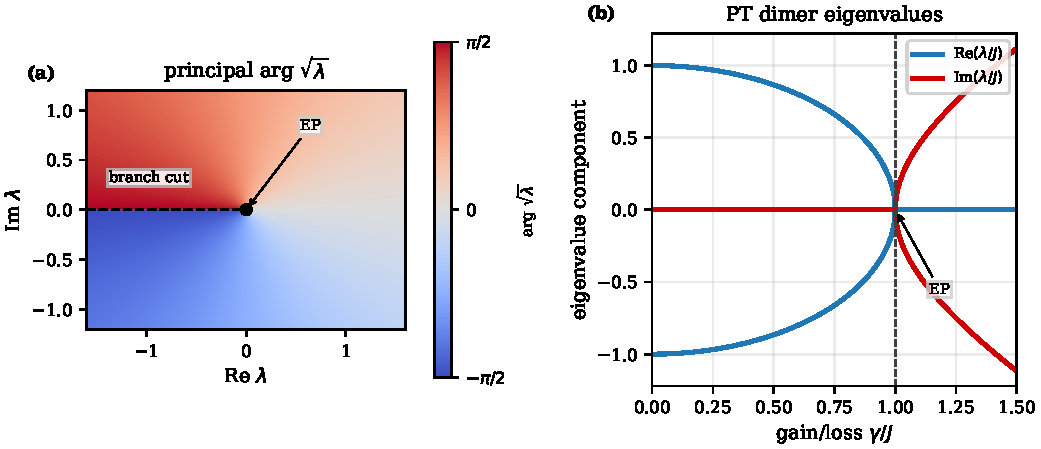
\includegraphics[width=\textwidth]{figures/fig_ch17_exceptional_riemann_step178.pdf}
  \caption{Exceptional-point branch-point topology.
  (a)~Principal argument $\mathrm{Arg}(\sqrt{\lambda})\in(-\pi/2,\,\pi/2]$
  over the complex $\lambda$-plane; the dashed line marks the branch cut on the
  negative real axis and the black dot is the EP at the origin.  The diverging
  \texttt{coolwarm} colour map is centred at zero phase.
  (b)~Eigenvalue components of the PT-symmetric dimer, normalised by the
  coupling~$J$.  Blue: real part; red: imaginary part.  Below the EP
  ($\gamma/J<1$) the spectrum is purely real; above it the spectrum is purely
  imaginary.  The dashed vertical line marks the EP at $\gamma/J=1$.}
  \label{fig:ch17-ep-riemann}
\end{figure}

\section{Non-Hermitian band topology}
\label{sec:ch17-nh-topology}

\subsection{Complex band structure}
\label{sec:ch17-complex-bands}

In a periodic non-Hermitian medium, the Bloch eigenfrequencies
$\omega_n(\kvec)=\omega_n'(\kvec)-\ii\gamma_n(\kvec)$ trace surfaces
in the complex $\omega$-plane as $\kvec$ varies.  The real part gives
the dispersion; the imaginary part gives the spatially resolved loss or
gain profile.

Two bands can coalesce not only in frequency but also in their loss
rates, forming \emph{exceptional lines} (1D curves in $\kvec$-space)
or \emph{exceptional surfaces} (2D surfaces in $\kvec$-space).  These
are topological objects in their own right, characterised by the
discriminant winding number.

\subsection{The non-Hermitian Chern number} \cite{unknown2018phys}
\label{sec:ch17-nh-chern}

A Chern number can still be defined using the biorthogonal Berry
connection \eqref{eq:ch17-nh-berry}:
\begin{equation}\label{eq:ch17-nh-chern}
  \Chern_n^{\mathrm{NH}} = \frac{1}{2\pi}\int_\BZ
  \bigl(\partial_{k_x}\Aberry_{n,y}^{\mathrm{NH}}
  - \partial_{k_y}\Aberry_{n,x}^{\mathrm{NH}}\bigr)\dd^2k\,.
\end{equation}
Under certain conditions (the band remains non-degenerate with no
EP crossings in the BZ), this is still an integer.  However, when
exceptional points are present in the Brillouin zone, the Chern number
may not be well defined for individual bands, because the band labels
exchange at each EP.

In such cases, the \emph{composite} Chern number of all bands involved
in the EP remains well defined, similar to the composite Chern number
for degenerate bands in the Hermitian case.

\subsection{The non-Hermitian skin effect}
\label{sec:ch17-skin}

A striking non-Hermitian phenomenon with no Hermitian analog is the
\emph{non-Hermitian skin effect} (NHSE)
\cite{lee2016anomalous,price2022roadmap,yao2018edgea}: in certain non-Hermitian
lattice systems, \emph{all} eigenstates are localised at one boundary
of the system under open boundary conditions, even though the bulk band
structure (computed with periodic boundary conditions) predicts extended
states.

\paragraph{Origin.}
The NHSE arises from asymmetric hopping: if the hopping amplitude for
rightward motion $J_R$ differs from the leftward amplitude $J_L$, there
is a net ``probability current'' that drives all modes toward one edge.
In the simplest model (Hatano--Nelson):
\begin{equation}\label{eq:ch17-hatano-nelson}
  H = \sum_n\bigl(J_R\,c_{n+1}^\dagger c_n
  + J_L\,c_n^\dagger c_{n+1}\bigr)\,,
\end{equation}
with $J_R\neq J_L$
\cite{lin2023topological}.  Under periodic boundary conditions, the spectrum
is a closed curve in the complex plane.  Under open boundary conditions,
all eigenstates are exponentially localised at the left (or right)
boundary, with localisation length $\xi=a/|\ln(J_R/J_L)|$.

\paragraph{Consequence for topology.}
The NHSE invalidates the conventional bulk-edge correspondence:
the Bloch Chern number (computed with periodic boundary conditions)
does not correctly predict the number of edge modes under open
boundary conditions.

\subsection{The generalised Brillouin zone}
\label{sec:ch17-gbz}

To restore the bulk-edge correspondence in the presence of the NHSE,
one must replace the standard Brillouin zone (where $\kvec$ is real)
with the \emph{generalised Brillouin zone} (GBZ), where $\kvec$ is
allowed to be complex:
\begin{equation}\label{eq:ch17-gbz}
  k = k' + \ii\kappa\,,\qquad \kappa\neq 0\,.
\end{equation}
The imaginary part $\kappa$ accounts for the exponential localisation
of the skin modes.  The non-Bloch Chern number, computed on the GBZ,
correctly predicts the number and direction of topological edge modes
\cite{kunst2018biorthogonal}.

\subsection{The non-Bloch bulk-boundary correspondence}
\label{sec:ch17-non-bloch}

In Hermitian systems, the bulk-edge correspondence relates the number
of edge modes to Chern numbers computed from Bloch bands with real
wavevector $k$.  In non-Hermitian systems with the skin effect, this
correspondence breaks down: the Bloch-band Chern number may predict a
different number of edge modes than what actually exists
\cite{lee2016anomalous,gong2018topologicala}.

The resolution is the \emph{generalised Brillouin zone} (GBZ): instead
of restricting $k$ to the real axis, one allows $k$ to take complex
values $k=k_R+\ii k_I$, with $k_I$ determined self-consistently by
requiring that the eigenstates be normalisable in a semi-infinite
system.  The locus of these complex $k$ values traces out a curve in
the complex $k$-plane---the GBZ---which replaces the standard BZ.

The non-Bloch Chern number is defined by integrating the Berry
curvature over the GBZ:
\begin{equation}\label{eq:ch17-non-bloch-chern}
  \Chern_{\mathrm{GBZ}}
  = \frac{1}{2\pi}\oint_{\mathrm{GBZ}}
  \Omega_n(\beta)\,\dd\beta\,,
\end{equation}
Here, $\beta$ parametrises the GBZ.  This non-Bloch invariant
correctly predicts the number of edge modes in all known examples,
restoring a modified bulk-edge correspondence.

\begin{figure}[t]
  \centering
  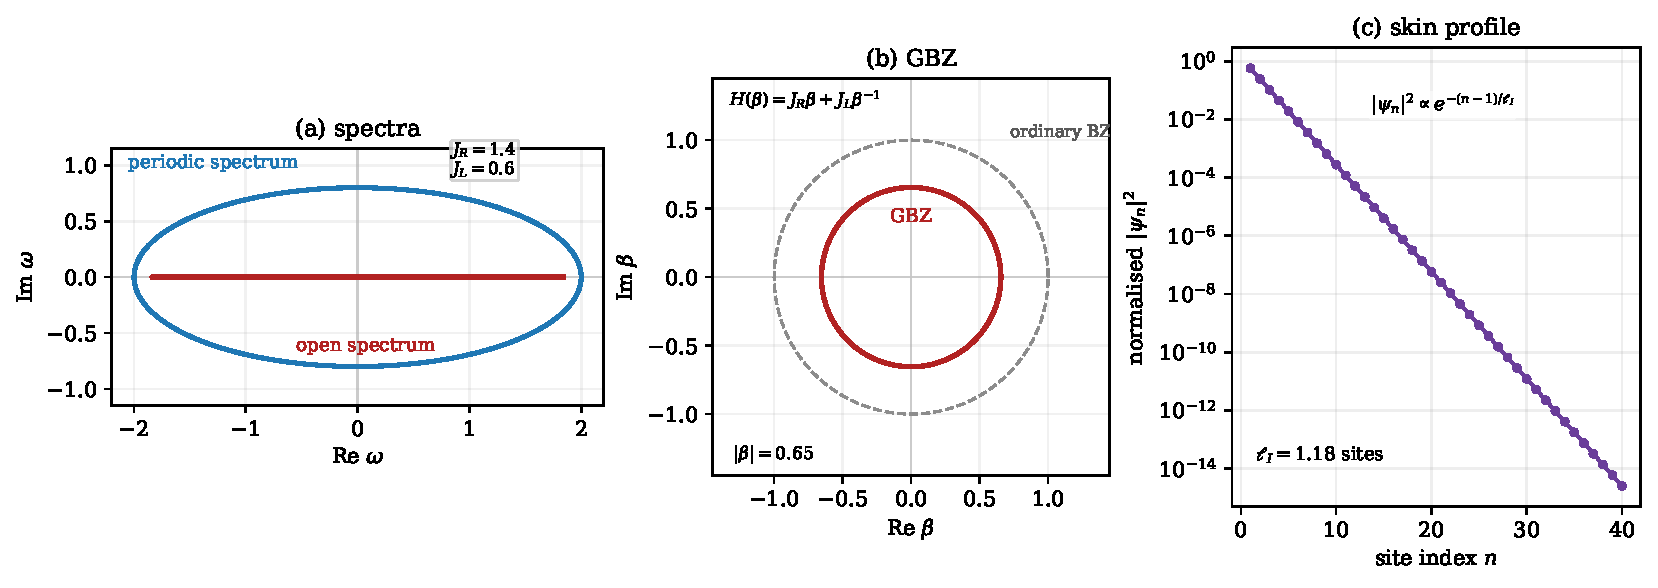
\includegraphics[width=\textwidth]{figures/fig_nonhermitian_skin_gbz.pdf}
  \caption{The Hatano--Nelson model with asymmetric hopping
    $J_R=1.4$, $J_L=0.6$.
    \textbf{(a)}~Complex-frequency spectra: with periodic boundaries
    the eigenvalues form an ellipse (blue); with open boundaries they
    collapse onto the real axis (red), a hallmark of the
    non-Hermitian skin effect.
    \textbf{(b)}~The generalised Brillouin zone (GBZ, red circle)
    has radius $|\beta|=\sqrt{J_L/J_R}\approx 0.65$, smaller than
    the unit circle of the ordinary BZ (dashed).  The dispersion
    relation is $H(\beta)=J_R\beta+J_L\beta^{-1}$.
    \textbf{(c)}~Normalised intensity profile
    $|\psi_n|^2\propto\ee^{-(n-1)/\ell_I}$ with intensity decay
    length $\ell_I=1/\ln(J_R/J_L)\approx 1.18$ sites, confirming
    that all eigenstates are exponentially localised at one boundary.}
  \label{fig:ch17-hatano-nelson}
\end{figure}

\subsection{Hatano--Nelson model}
\label{sec:ch17-hatano-nelson}

The simplest model exhibiting the skin effect is the Hatano--Nelson
chain with asymmetric hopping $J_L\neq J_R$:
\begin{equation}\label{eq:ch17-hatano-nelson-ket}
  H = \sum_n\bigl(J_R\,|n{+}1\rangle\langle n|
  + J_L\,|n\rangle\langle n{+}1|\bigr)\,.
\end{equation}
With periodic boundaries, the eigenvalues form an ellipse in the
complex plane: $\omega(k)=J_R\ee^{\ii k}+J_L\ee^{-\ii k}$.  With
open boundaries, \emph{all} eigenstates localise at one end, and the
eigenvalues collapse onto a real interval.  The GBZ is a circle of
radius $|\beta|=(J_L/J_R)^{1/2}$, deformed from the unit circle of
the standard BZ.  For the intensity profile plotted in
\figref{fig:ch17-hatano-nelson},
\begin{equation}
  |\psi_n|^2 \propto \exp[-(n-1)/\ell_I] ,
  \qquad
  \ell_I=\frac{1}{|\ln(J_R/J_L)|}\,.
\end{equation}
This is the intensity skin length; the field-amplitude decay length is
larger by a factor of two for the same convention.

A photonic implementation uses coupled resonators with unidirectional
coupling via gain/loss engineering \cite{price2022roadmap}.

\section{PT-symmetric photonic systems}
\label{sec:ch17-pt}

\subsection{PT symmetry in photonics}
\label{sec:ch17-pt-photonics}

A particularly important class of non-Hermitian photonic systems has
$\PT$ symmetry \cite{longhi2018parity}: the combined parity-time
symmetry requires balanced loss and gain:
\begin{equation}\label{eq:ch17-pt-condition}
  \varepsilon(\rvec) = \varepsilon^*(-\rvec)\,.
\end{equation}
This means: the real part of $\varepsilon$ is even ($\varepsilon'(\rvec)
=\varepsilon'(-\rvec)$), and the imaginary part is odd
($\varepsilon''(\rvec)=-\varepsilon''(-\rvec)$).

When $\PT$ symmetry is unbroken (below the EP threshold), the
eigenfrequencies are real despite the non-Hermiticity.  The $\PT$ phase
transition---from real to complex eigenfrequencies---occurs at an
exceptional point where the gain/loss parameter exceeds the coupling
strength.

\subsection{PT-symmetric photonic lattices}
\label{sec:ch17-pt-lattices}

$\PT$-symmetric photonic lattices can be constructed by alternating
lossy and amplifying elements:
\begin{itemize}
  \item Coupled waveguides with alternating gain and loss.
  \item Microring resonator arrays with alternating pump and
  absorption.
  \item Photonic crystal defect cavities with controlled $Q$-factor
  modulation.
\end{itemize}
These systems exhibit $\PT$ phase transitions, unidirectional
invisibility, and enhanced sensing near exceptional points
\cite{ozawa2018topological}.

\section{Topological lasers}
\label{sec:ch17-lasers}

\subsection{Principle of operation}
\label{sec:ch17-laser-principle}

A topological laser combines topological photonics with optical gain to
create a laser whose mode structure is determined by topological edge
states
\cite{harari2018topological,bandres2018topologicalb}.  The key idea is:
\begin{enumerate}
  \item Fabricate a photonic system with topological edge modes.
  \item Provide optical gain (by electrical or optical pumping).
  \item The topological edge mode lases preferentially because:
  \begin{itemize}
    \item It samples the gain region over a large spatial extent.
    \item It is spectrally isolated within the topological gap.
    \item Backscattering is suppressed, enhancing the effective
    cavity $Q$.
  \end{itemize}
\end{enumerate}

\subsection{Experimental demonstrations}
\label{sec:ch17-laser-demos}

Topological lasers have been demonstrated in several platforms:

\paragraph{1D SSH laser arrays.}
Chains of coupled microring lasers with alternating coupling, where
the topological edge mode at the SSH domain wall lases preferentially.
The edge-mode laser shows single-mode operation over a wide pump range,
while the corresponding trivial array shows multi-mode behaviour.

\paragraph{2D topological insulator lasers.}
Arrays of coupled ring resonators forming a 2D topological photonic
system (Hafezi-type), where the edge-mode laser wraps around the
entire boundary \cite{zhu2026topology}.  The lasing is coherent around the boundary and
robust to deliberate defects.

\paragraph{Valley-Hall lasers.}
Photonic crystal slab lasers using valley-Hall edge modes in III--V
semiconductor platforms, demonstrating single-mode lasing along
designed domain-wall paths.

\section{What survives from the Hermitian theory}
\label{sec:ch17-survives}

\begin{center}
\begin{tabular}{lll}
  \toprule
  \textbf{Hermitian} & \textbf{Non-Hermitian} & \textbf{Status} \\
  \midrule
  Real $\omega_n$ & Complex $\omega_n$ & Always \\
  Orthogonal modes & Biorthogonal modes & Always \\
  $\langle f|\Mmat|g\rangle$ positive & Indefinite & Always \\
  Dirac points & Exceptional points & Different codimension \\
  Chern number $\in\mathbb{Z}$ & NH Chern number $\in\mathbb{Z}$
    & If no EP in BZ \\
  Standard BEC & Modified (GBZ needed) & If skin effect present \\
  No backscatter & No backscatter & Survives \\
  Lossless propagation & Lossy/amplified & Does not survive \\
  \bottomrule
\end{tabular}
\end{center}

The most important message: topological protection against
\emph{backscattering} survives in non-Hermitian systems (the edge mode
still has no counter-propagating partner within the gap), but protection
against \emph{loss} does not.  A topological edge mode in a lossy
system decays as it propagates; it simply does so without reflecting.

\section{The PT phase transition in coupled waveguides}
\label{sec:ch17-pt-lattices-experiment}

Parity-time (PT) symmetric systems have balanced gain and loss
arranged so that the Hamiltonian commutes with the combined PT
operator.  In photonics, this translates to a refractive index profile
with $n(\rvec)=n^*(-\rvec)$: the real part is symmetric and the
imaginary part (gain/loss) is antisymmetric.

\subsection{The PT phase transition}
\label{sec:ch17-pt-transition}

Below a critical gain/loss strength $\gamma_{\mathrm{PT}}$, the
eigenfrequencies are real despite the non-Hermitian Hamiltonian---this
is the PT-symmetric (unbroken) phase.  Above $\gamma_{\mathrm{PT}}$,
eigenfrequencies become complex conjugate pairs, signalling the
spontaneous breaking of PT symmetry.  The transition occurs at an
exceptional point where two eigenstates coalesce
\cite{guo2009observation,peng2014loss}.

Guo et~al.\ (2009) observed this transition in a pair of coupled
optical waveguides, one with gain (pumped erbium-doped fibre) and one
with loss (chromium-coated fibre).  The transition manifested as a
sharp change in the transmission spectrum from symmetric doublet
splitting (PT-unbroken) to exponential growth/decay
(PT-broken) \cite{guo2009observation}.

\subsection{Loss-induced lasing and PT-symmetric lasers}
\label{sec:ch17-pt-laser}

A remarkable consequence of PT symmetry is that adding loss can
\emph{increase} the output of a laser.  Peng et~al.\ (2014)
demonstrated this using two coupled whispering-gallery-mode
microresonators: one actively pumped and one with controllable loss
introduced by a chromium nanotip.  As the loss was increased, the
system passed through an exceptional point, and the lasing power
first decreased and then \emph{revived}, exceeding its initial value
\cite{peng2014loss}.

This counterintuitive effect occurs because the exceptional point
redistributes the mode energy: in the PT-broken phase, the lasing
mode is concentrated in the gain resonator, reducing its overlap with
the lossy resonator and effectively increasing the net gain.

\section{Topological lasing and nonlinear stability}
\label{sec:ch17-topological-laser}

The combination of non-Hermitian physics and topology has led to the
concept of a \emph{topological laser}: a laser whose mode is a
topological edge state, protected against backscattering and disorder \cite{elganainy2018non}.

The first topological laser was demonstrated using a ring of coupled
microring resonators with one-way edge modes pumped above threshold.
The topological protection ensures single-mode lasing: the edge mode
has a longer round-trip path and lower lasing threshold than competing
bulk modes, and it is robust against fabrication imperfections that
would otherwise cause mode hopping or multi-mode oscillation
\cite{ozawa2018topological,price2022roadmap}.

A key theoretical question is whether the topological protection
survives in the nonlinear regime above threshold.  Above the lasing
threshold, gain saturation introduces an intensity-dependent
refractive index that can break the symmetries protecting the
topological mode.  Current evidence suggests that the protection
persists for moderate pumping but can break down at very high pump
powers \cite{li2022gain,zhu2020photonic}.

\section{Non-Hermitian topological classification}
\label{sec:ch17-classification}

The classification of topological phases in non-Hermitian systems is
fundamentally richer than in the Hermitian case \cite{kawabata2019classification}.  The key distinction
is between \emph{line gaps} (no eigenvalue crosses a reference line
in the complex plane) and \emph{point gaps} (no eigenvalue reaches a
reference point).  These two gap types lead to different topological
invariants \cite{gong2018topologicala}.

For line-gapped systems, the classification reduces to the Hermitian
tenfold way, and the Chern number remains a valid topological
invariant.  For point-gapped systems, new invariants appear,
including winding numbers that count the number of times the complex
eigenvalue spectrum winds around the reference point as the Bloch
momentum traverses the Brillouin zone.

The full non-Hermitian classification contains 38 symmetry classes
(compared to 10 in the Hermitian case), because the transpose and
complex conjugate operations are no longer equivalent for non-Hermitian
matrices.  This enriched classification predicts topological phases
that have no Hermitian counterpart, such as the non-Hermitian skin
effect discussed in Section~\ref{sec:ch17-skin}
\cite{gong2018topologicala,lee2016anomalous}.

\section{The non-Hermitian skin effect in higher dimensions}
\label{sec:ch17-skin-higher-dim}

The non-Hermitian skin effect (NHSE), discussed in
Section~\ref{sec:ch17-skin} for 1D, generalises to higher dimensions
with qualitatively new features.

\subsection{Hybrid skin-topological effect}
\label{sec:ch17-hybrid}

In a 2D non-Hermitian system with both nonzero Chern number and
asymmetric hopping, the bulk modes can localise at one edge (the skin
effect) while the topological edge modes localise at a corner (where
the skin edge meets the topological edge).  This \emph{hybrid
skin-topological effect} was predicted by Li et~al.\ (2022) in a
non-Hermitian Haldane model with balanced gain and loss on different
sublattice sites \cite{li2022gain}.

The corner-localised modes have a unique character: they inherit the
unidirectional propagation of the topological edge and the exponential
localisation of the skin effect, creating a new type of higher-order
topological state that exists only in non-Hermitian systems.

\subsection{Photonic observation of the skin effect}
\label{sec:ch17-skin-photonic}

Zhu et~al.\ (2020) proposed a photonic implementation of the NHSE
using a 1D chain of coupled resonant optical waveguides (CROWs) with
asymmetric coupling.  The asymmetry is achieved by introducing
auxiliary waveguides that mediate different coupling strengths for
clockwise and counter-clockwise propagation.  The predicted skin
localisation length is $\ell_{\mathrm{skin}}=1/\ln|J_R/J_L|$,
where $J_R$ and $J_L$ are the rightward and leftward hopping
amplitudes \cite{zhu2020photonic,lee2016anomalous}.

The non-Bloch Chern number for this system is computed using the
generalised Brillouin zone (GBZ, Section~\ref{sec:ch17-gbz}), and
it correctly predicts the number of topological edge modes even when
the conventional Bloch Chern number fails
\cite{gong2018topologicala,zhu2020photonic}.

\section{Topological insulator lasers}
\label{sec:ch17-topological-lasers}

Perhaps the most compelling application of non-Hermitian topological
photonics is the \emph{topological insulator laser}: a laser array
in which the lasing mode is a topologically protected edge state,
inheriting the robustness of topological transport.

\subsection{Theoretical framework}
\label{sec:ch17-ti-laser-theory}

The theoretical foundation for topological insulator lasers was
established by Harari et~al.\ (2018), who showed that a
two-dimensional lattice of coupled ring resonators with optical gain
on the edge and loss in the bulk can support single-mode lasing in
a topological edge state \cite{harari2018topological}.

The governing equation for the slowly varying amplitude $a_n$ at
site $n$ is
\begin{equation}\label{eq:ch17-laser-amplitude}
  \ii\frac{\dd a_n}{\dd t}
  = \sum_m J_{nm}\,a_m
  + \bigl(g_n - \gamma_n\bigr)a_n
  - g_n^{(2)}|a_n|^2\,a_n\,,
\end{equation}
where $J_{nm}$ is the coupling between resonators $n$ and $m$,
$g_n$ is the linear gain, $\gamma_n$ is the linear loss, and
$g_n^{(2)}$ is the gain saturation coefficient.  The gain is
confined to the edge resonators: $g_n>0$ for edge sites and
$g_n=0$ for bulk sites.

The key insight is that the topological edge mode has the largest
spatial overlap with the gain region.  Above the lasing threshold,
the edge mode is the first to reach positive net gain
$(g_n-\gamma_n>0)$ and saturates the gain for all other modes,
producing stable single-mode lasing.  Competing bulk modes, which
have most of their intensity in the lossy bulk, remain below
threshold \cite{harari2018topological,ozawa2018topological}.

\subsection{Experimental demonstration}
\label{sec:ch17-ti-laser-experiment}

The topological insulator laser was demonstrated experimentally by
Bandres et~al.\ (2018) using a $10\times 10$ array of coupled ring
resonators fabricated on an InGaAsP quantum-well platform
\cite{bandres2018topologicala}.  The array implemented a
two-dimensional anomalous Floquet topological insulator lattice,
with the synthetic magnetic flux provided by spatially shifted link
resonators (phase parameter $\alpha=0.25$).

Optical pumping was applied selectively to the edge resonators using
a shaped pump beam.  Above threshold, the device exhibited
single-frequency lasing with a narrow linewidth, in contrast to a
topologically trivial array of the same size, which showed
multi-mode lasing with broad spectral output.  The slope efficiency
of the topological laser was found to increase with system size (as
more edge resonators contributed coherently), while the trivial
laser's efficiency decreased due to mode competition
\cite{bandres2018topologicala,harari2018topological}.

The topological protection manifested as robustness against
intentional defects: when one or two edge resonators were
deliberately detuned or blocked, the lasing mode rerouted around the
defect with minimal change in output power and linewidth.  This
behaviour is impossible in a conventional laser array, where defects
create scattering losses and mode distortions.

\subsection{Towards electrically pumped topological lasers}
\label{sec:ch17-electrical-pumping}

The initial demonstrations used optical pumping, which limits
practical applications.  Subsequent work has pursued electrically
pumped topological lasers in III-V semiconductor platforms, where
the challenge is to maintain the required coupling phases and gain
distribution with standard epitaxial fabrication techniques.

Preliminary results have shown that the topological protection
survives in the presence of the fabrication disorder inherent to
electrical injection ($\sim 5$\% variation in resonator frequencies),
and that the single-mode lasing persists over a range of pump
currents above threshold
\cite{ozawa2018topological,price2022roadmap}.  These developments
point toward scalable topological laser arrays for applications in
optical communication, sensing, and integrated photonics.

\section{Exceptional points and their photonic topology}
\label{sec:ch17-exceptional-points}

Exceptional points (EPs) are the hallmark degeneracies of
non-Hermitian systems: points in parameter space where two or more
eigenvalues \emph{and} their eigenvectors coalesce.  Unlike Hermitian
degeneracies (diabolic points), where the eigenvectors remain linearly
independent, at an EP the eigenvector space collapses and the
Hamiltonian becomes non-diagonalisable.

\subsection{The square-root topology of a second-order EP}
\label{sec:ch17-ep2-topology}

The simplest exceptional point is of second order (EP2), where two
eigenvalues coalesce.  Near an EP2 in a two-dimensional parameter
space $(p_1,p_2)$, the eigenvalue splitting behaves as
\begin{equation}\label{eq:ch17-ep2-splitting}
  \Delta\omega \propto \sqrt{(p_1-p_1^{(\mathrm{EP})})
  + \ii(p_2-p_2^{(\mathrm{EP})})}\,.
\end{equation}
The square-root branch point means that encircling the EP in parameter
space exchanges the two eigenvalues: after one loop, the system
returns to its starting point but with the two modes swapped.  This
eigenvalue exchange is a topological property of the EP and is robust
against perturbations that do not destroy the EP itself
\cite{ding2022non,kawabata2019classification}.

In photonic systems, EPs occur naturally when gain and loss are
balanced ($\PT$-symmetric systems) or when two resonances with
different lifetimes are coupled.  The eigenvalue exchange around an EP
has been observed experimentally in coupled microring resonators,
microwave cavities, and photonic crystal slabs
\cite{longhi2018parity,chong2010symmetry}.

\subsection{Higher-order exceptional points}
\label{sec:ch17-higher-ep}

Exceptional points of order $p$ (EP$p$), where $p$ eigenvalues
coalesce simultaneously, exhibit $p$th-root branch-point topology:
encircling the EP cyclically permutes all $p$ eigenvalues.  The
eigenvalue splitting near an EP$p$ scales as
$\Delta\omega \propto \epsilon^{1/p}$, where $\epsilon$ is the
distance from the EP in parameter space.

This enhanced sensitivity ($1/p$th-root response) has attracted
interest for sensing applications: an EP$p$ sensor responds to a
small perturbation $\epsilon$ with a frequency splitting proportional
to $\epsilon^{1/p}$, which can be much larger than the linear
response of a conventional sensor when $\epsilon$ is small.  However,
the practical utility of EP-enhanced sensing remains debated because
the same non-Hermitian physics that enhances the signal also
enhances the noise \cite{wang2020petermann,ding2022non}.

\subsection{Exceptional surfaces and lines}
\label{sec:ch17-exceptional-surfaces}

In three-dimensional parameter spaces, EPs generically form lines
(exceptional lines or rings) rather than isolated points.  In
photonic crystals with gain or loss, these exceptional lines can
thread through the Brillouin zone, creating non-Hermitian analogs
of nodal lines in Hermitian semimetals.

The intersection of exceptional lines with Weyl points produces
exotic objects called ``exceptional Weyl points,'' where the Weyl
point splits into a ring of EPs in the complex-frequency plane.  This
has been predicted for 3D photonic crystals with balanced gain and
loss and connects to the broader program of non-Hermitian Weyl
semimetal physics \cite{yang2019non,wang2021topological}.

\section{Photonic implementations of the non-Hermitian skin effect}
\label{sec:ch17-photonic-skin}

The non-Hermitian skin effect (NHSE)---the exponential localisation
of all eigenstates at one boundary under open boundary
conditions---has been observed in several photonic platforms.

\subsection{Non-reciprocal waveguide arrays}
\label{sec:ch17-skin-waveguide}

The simplest photonic implementation of the Hatano--Nelson model uses
an array of coupled waveguides with asymmetric coupling: the
coupling from waveguide $n$ to $n+1$ differs from the coupling from
$n+1$ to $n$.  This non-reciprocity can be achieved by coupling
through an intermediate waveguide with gain on one side and loss on
the other, or by using magneto-optical materials that provide
non-reciprocal coupling \cite{longhi2019probing,okuma2020topological}.

Weidemann et~al.\ (2020) demonstrated the NHSE in a
discrete-time photonic quantum walk using fibre loops with
asymmetric coupling, observing the predicted exponential localisation
of all modes at one boundary, with a skin length consistent with the
non-Bloch theory prediction
$\xi_{\mathrm{skin}} = 1/\ln|J_R/J_L|$
\cite{okuma2020topological,imura2020generalized}.

\subsection{Topological lasers and the NHSE}
\label{sec:ch17-topo-laser}

The intersection of topological edge states and non-Hermitian physics
has produced a new class of devices: topological lasers.  In a
topological laser, the gain medium is placed along the edge of a
photonic topological insulator, and the lasing mode is a topological
edge state protected from backscattering by the bulk topology.

Bandres et~al.\ (2018) demonstrated the first topological insulator
laser using a 2D array of coupled microring resonators
\cite{bandres2018topologicalb,harari2018topological}.  The key
advantage over conventional laser arrays is that the topological
edge mode maintains its spatial coherence even in the presence of
fabrication disorder, because the one-way nature of the edge state
prevents the formation of localised lasing hot spots.

More recently, topological lasers have been realised in valley
photonic crystals \cite{zhu2026topology} and photonic crystal slabs
operating at bound states in the continuum (BICs), where the
topological protection of the BIC mode suppresses radiation losses
and lowers the lasing threshold
\cite{price2022roadmap}.

\section*{Exercises}

\begin{exercise}
  For the coupled-resonator Hamiltonian \eqref{eq:ch17-coupled-resonators}
  with $\omega_1=\omega_2=\omega_0$, $\gamma_1=-\gamma_2=\gamma$
  ($\PT$-symmetric case), find the exceptional point in the $(J,\gamma)$
  plane.  Show that the eigenvalues are real for $J>|\gamma|/2$ and
  complex for $J<|\gamma|/2$.
\end{exercise}

\begin{exercise}
  Show that encircling an exceptional point in parameter space causes
  the two eigenvalues to exchange.  \emph{Hint:} parametrise a loop
  around the EP using $\delta=\rho\ee^{\ii\phi}$ in
  \eqref{eq:ch17-ep-splitting} and track $\omega_\pm$ as
  $\phi:0\to 2\pi$.
\end{exercise}

\begin{exercise}
  For the Hatano--Nelson model \eqref{eq:ch17-hatano-nelson} with
  $J_R=2$, $J_L=1$, and $N=20$ sites: (a) compute the spectrum under
  periodic boundary conditions, (b) compute the spectrum under open
  boundary conditions, and (c) show that all open-boundary eigenstates
  are exponentially localised at the left edge.
\end{exercise}

\begin{exercise}
  The biorthogonal Berry connection \eqref{eq:ch17-nh-berry} is
  generally complex.  Show that its imaginary part equals
  $\partial_{k_a}\ln|N_n(\kvec)|/(2\ii)$, where
  $N_n=\langle\mathbf{u}_n^L|\Mmat|\mathbf{u}_n^R\rangle$ is the
  biorthogonal norm.
\end{exercise}

\begin{exercise}
  A topological laser has an edge mode with group velocity $v_g$,
  topological gap $\Delta\omega$, round-trip length $L$, and material
  gain coefficient $g_0\;\mathrm{cm}^{-1}$.  (a) Estimate the lasing
  threshold $g_{\mathrm{th}}$ in terms of the out-coupling loss and
  any residual absorption.  (b) Compare the threshold with a
  conventional Fabry--P\'erot laser of the same length, explaining why
  the topological laser can have a lower threshold.
\end{exercise}

\begin{exercise}
  Show that the $\PT$ condition $\varepsilon(\rvec)=\varepsilon^*(-\rvec)$
  for a 1D photonic crystal with period $a$ requires the real part of
  $\varepsilon$ to be even and the imaginary part to be odd under
  $x\to-x$ \cite{zhong2021non}.  Design a unit cell with two layers satisfying this
  condition.
\end{exercise}
